%-----------------------------------------------------------------------------------------
\clearpage
\section{Implementation}
%-----------------------------------------------------------------------------------------

\subsection{Tooling}
Implementing a distributed neural network is too large a task to be undertaken
from scratch. Therefore its necessary to used existing tools, to make the
development viable in the time given. This is difficult as not many languages
lend themselves to both distributed systems and neural networks.

To ensure high performance the project could be implemented in C++. While C++ is
often very performant and also has low level bindings for ML libraries such as
TensorFlow. However even the creator of the language sees the need to improve
its ability to improve its distributed performance. \cite{stroustrupInterview}

Python has great tooling for neural networking, such as TensorFlow
\cite{abadi2016tensorflow}, and PyTorch \cite{paszke2019pytorch}. Moreover it
has great support for numerical computing with NumPy \cite{harrisNumpy2020}.
These are performant too, by calling C functions or creating code which is
optimised to run on GPUs to parallelise computation. However due to the Global
Interpreter Lock (GIL) python is infamously bad at concurrency, while its
distributed tooling is implemented in native python code, which lack of speed
and could bottleneck the performance gained from using NumPy and TensorFlow.

Ultimately I decided to use Elixir as the programming language of
implementation. This is because Elixir was designed for developing highly
concurrent distributed systems. It does this by having a uniquely brilliant
concurrency model. As opposed to OOP languages where 'everything is an object'
in Elixir 'everything is a process'. This means the default way of writing the
language enables it to be concurrent and scalable. Elixir also has the ability
to communicate with other Elixir programs over the network using its own
application protocol on top of TCP/IP. Meaning its as easy to communicate with
local processes on your own machine as processes on another machine running an
Elixir program. Its also been used by artificial intelligence researchers before
as the process concurrency models effortlessly lends itself to modelling
neurons. \cite{sherNeuroevolutionThroughErlang} Using Elixirs native float and
arithmetic implementation would be slower than a C++ or a NumPy implementation,
luckily there is a stable package which supports matrix calculations even faster
than those in NumPy called Matrex. \cite{matrex}

The only drawback of using Elixir is at the time of development it didn't have a
strong machine learning library, which means implementing the mathematics of the
neural network myself. While this was a sizeable amount of work to do, it had
the benefit that I didn't to wrestle with an opinionated API such as TensorFlow,
I could create my own API to meet my ends.

\subsection{Neural Network Implementation}
In order to create a distributed neural network. I first needed to create a
basic feed forward network that could operate on a single machine. This network
didn't need to be fully featured, its just a means to make an objectively
comparative performance between RingTMP and a generic parameter server.
Therefore only 2 types of layers were implemented, the hidden layer and the
output layer. The hidden layer is a generic dense layer similar to the kind you
would find in any other neural network library. The output layer performs
similarly to the hidden layer with the key difference that its always the final
layer and outputs the activations as probabilities. Within this section I will
explain in more detail how the neural network was implemented from scratch and
the mathematics behind its function.

% creating a network should go here first
\subsubsection{Initialisation}
Neural networks are composed of layers, while conceptually layers are
composed of neurons, they're practically implemented with two components. A
weights matrix and a bias vector. As I have already mentioned in this network
there are two types of layers, hidden layers and output layers. We need to label
each layer with its type, so we know how to perform the forward and
backpropagation. Therefore we can describe a layer as the tuple:
\begin{lstlisting}[numbers=none,frame=none]
    {layer_type, weights, bias}
\end{lstlisting}

Placing several of these tuples in a list creates a network:
\begin{lstlisting}[numbers=none,frame=none]
  [{:hidden_layer, weights_1, bias_1},
   {:hidden_layer, weights_2, bias_2},
   {:output_layer, weights_3, bias_3}]
\end{lstlisting}

The weights and biases have different dimensions depending on the layers input size
and output size. A layer might take an activations vector with a size of \(m\) and
output a size of \(n\). The layer would hold a \(n \times m\) matrix
and the dimensions of the bias would be \(n \times 1\). The
output size of one layer must be the input size of the next layer, else the
network will fail to function.

Initialising the biases is simple, as biases have the function of an intercept
in a linear equation, they can be initialised to 0. The trivial code is below:
\begin{lstlisting}
  defp initialise_bias(col) do
    Matrex.zeros(col, 1)
  end
  \end{lstlisting} 

Weights are more complex. Each layer is initialised with random values from a
uniform distribution, the shape of the uniform distribution is dependant upon
the size of the input and output layers of the neural network. The type of
initialisation used is dependant upon the activation function used.

In the hidden layer the ReLU function is used, common wisdom first established
in this paper \cite{he2015delving} states that for the fastest convergence He
initialisation should be used. He initialisation is done by sampling random
values from a normal distribution with a mean of 0 and a variance of \( 2/N \)
where \(N\) represents the number of input values to a layer.

For the output layer, the softmax function is used. The best initialisation
method in this case is using Xavier
initialisation. \cite{glorot2010understanding} This also takes random samples
from a normal distribution with a mean of 0 but has the variance of \( 1/N \)
where \(N\) is \( (inputSize + outputSize) / 2 \).

However in practice training the model often failed with He initialisations.
This was because of what is know as the 'Dying ReLU Problem'. Which is when the
elements of the z vector of a layer are negative, the ReLU activation function
will return a zero meaning no learning is taking place. Once a neuron becomes
dead its unlikely it will be revived as the function is piecewise and provides
no slope for recovery such as a Leaky ReLU or a sigmoid function. To remedy this
I trialed many distributions, settling on a mean of 0.5 with a variance of 0.25.
While this is more simplistic, and may impact training times, its far more
likely for the network to not be dead on arrival because of the initialisation
parameters. This is part of the code which initialises the matrices in the layers:
\begin{lstlisting}
  defp random_val(_x, {n, :he, seed_state, acc}) do
    {val, new_state} = :rand.normal_s(0, 2 / col, seed_state)
    {col, :he, new_state, [val | acc]}
  end

  defp random_val(_x, {n, :pos, seed_state, acc}) do
    {val, new_state} = :rand.normal_s(0.5, 0.25, seed_state)
    {n, :pos, new_state, [val | acc]}
  end

  defp random_val(_x, {n, :xavier, seed_state, acc}) do
    {val, new_state} = :rand.normal_s(0, 1 / col, seed_state)
    {col, :xavier, new_state, [val | acc]}
  end
\end{lstlisting}

you can find the wider context for this code snippet in code listing in the Appendix 1. ~\ref{network_initialisation} 

\subsubsection{Forward Propagation}

% need to put this stuff earlier its already been explained
Neural networks are composed of layers, each layer is composed of neurons.
Numerical inputs are inserted through the input layer, forward propagate through
the network and push numerical results to the output layer. For our purposes
each neuron in the output layer represents a different category, the value of
that neuron is the probability the given input belongs to that category.

Each neuron holds a value, called an activation. Each layer has a bias and a
collection of neurons. Between the layers every neuron in one layer connects to
every other neuron in the next layer, every connection has an associated value
called a weight. To calculate the weight of a single neuron in the next layer
you must multiply the activations of the previous layer with the weights
connected to the neuron in question, then sum the values, add the bias, then
apply the activation function to that value. To explain more visually the
process and mathematics more visually, see the diagram below of the interaction
between two layers each with two nodes.

<<REDO THIS BIT ABOVE>>

\begin{figure}[h]
    \centering
    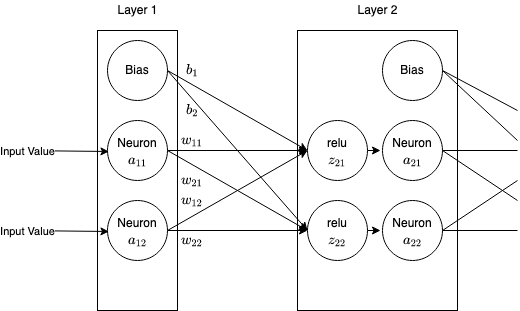
\includegraphics[width=0.6\textwidth]{two_neuron_network_1}
\end{figure}

\begin{equation}
    \begin{aligned}
        z_{21} &= a_{11}w_{11} + a_{12}w_{12} + b_{1} \, \, \, \, \, \, \, z_{22} = a_{11}w_{21} + a_{12}w_{22} + b_{2} \\
        a_{21} &= relu(z_{21}) \, \, \, \, \, \, \, a_{22} = relu(z_{22}) 
    \end{aligned}
\end{equation}


As networks become larger using this notation above becomes cumbersome. So we
use matrices to simplify the situation. Where \(X\) is the input matrix, \(W\)
is the weights, \(B\) is the bias, \(activationFunc(x)\) is the activation function and finally \(A\) is the output activation.

\begin{equation}
    \begin{aligned}
        X = \begin{bmatrix}
            a_{11} \\
            a_{12}
        \end{bmatrix} \, \, \, \, \, \, \,
        W &= \begin{bmatrix}
            w_{11} & w_{12} \\
            w_{21} & w_{22}
        \end{bmatrix} \, \, \, \, \, \, \,
        B = \begin{bmatrix}
            b_{1} \\
            b_{2}
        \end{bmatrix} \\[10pt]
        A &= activationFunc( W^{T}X + B)
    \end{aligned}
\end{equation}

In my implementation there are only two layer types. Hidden layers and output
layers. The only difference between these two layers is the activation function
that they use. Hidden layers use the ReLU activation function which is a simple
piecewise non-linear function described as such:
\begin{equation}
    relu(z) = max(0,z)
\end{equation}
This function has become the de facto application function in dense hidden
layers since its debut in 2011. \cite{glorot2011deep}. In Elixir the forward
action in the hidden layer is implemented like so: \footnote{The pipe operator
\lstinline{|>} transforms the function \lstinline{val_a |> a_function(val_b)}
into \lstinline{a_function(val_a, val_b)}}
\begin{lstlisting}
  def forward(previous_activation, weights, bias) do
    weights|> Matrex.transpose()
    |> Matrex.dot(previous_activation)
    |> Matrex.add(bias)
    |> relu()
  end

  defp relu(z_vector) do
    z_vector|> Matrex.apply(
        fn value, _index -> if value > 0, do: value, else: 0 end
    )
  end
\end{lstlisting}

The output layer uses a more complex activation function, the softmax function,
which transforms its inputs into probabilities. The sum of these probabilities
is always 1. This is the softmax function, where \(z\) is a \(i \times 1\)
vector:
\begin{equation}
    softmax(z)_{i} = \frac{e^{z_{i}}}{\sum_{j=1}^{n} e^{z_{j}}}
\end{equation}

This function is implemented the categorical output layer like so:
\begin{lstlisting}
    def forward(previous_activation, weights, bias) do
        weights|> Matrex.transpose()
        |> Matrex.dot(previous_activation)
        |> Matrex.add(bias)
        |> softmax()
    end

    defp softmax(z_vector) do
        stabilised_vec = Matrex.subtract(z_vector, Matrex.max(z_vector))
        exp = Matrex.apply(stabilised_vec, :exp)
        Matrex.divide(exp, Matrex.sum(exp))
    end
\end{lstlisting}

% show forward propagation function across the networks





% put equations here

% second diagram here
% second equations here

% $$a_{2} = relu(z)$$

% $$z = a_{1}w + b$$

% \begin{figure}[h]
%     \centering
%     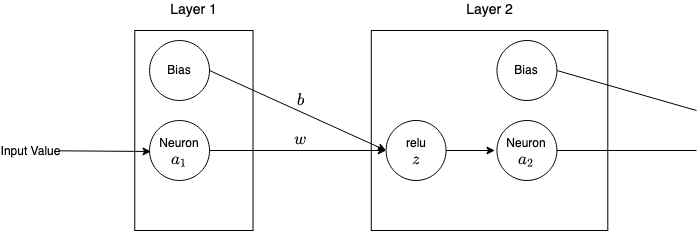
\includegraphics[width=0.6\textwidth]{simplest_neural_network_1}
% \end{figure}
% \begin{equation}
%     z_{21} = a_{11}w_{11} + a_{12}w_{12} + b_{1} \, \, \, \, \, \, \, z_{22} = a_{11}w_{21} + a_{12}w_{22} + b_{2}
% \end{equation}
% \begin{equation}
%     a_{21} = relu(z_{21}) \, \, \, \, \, \, \, a_{22} = relu(z_{22}) 
% \end{equation} 
% \begin{equation}
%     z = a_{1}w + b
% \end{equation}
% \begin{equation}
%     a_{2} = relu(z)
% \end{equation}

% The activation function being used
% in the hidden layers in this project is the ReLU function, which has become the de
% facto activation function since its discovery in 2011. \cite{glorot2011deep}
